\documentclass[1p]{elsarticle_modified}
%\bibliographystyle{elsarticle-num}

%\usepackage[colorlinks]{hyperref}
%\usepackage{abbrmath_seonhwa} %\Abb, \Ascr, \Acal ,\Abf, \Afrak
\usepackage{amsfonts}
\usepackage{amssymb}
\usepackage{amsmath}
\usepackage{amsthm}
\usepackage{scalefnt}
\usepackage{amsbsy}
\usepackage{kotex}
\usepackage{caption}
\usepackage{subfig}
\usepackage{color}
\usepackage{graphicx}
\usepackage{xcolor} %% white, black, red, green, blue, cyan, magenta, yellow
\usepackage{float}
\usepackage{setspace}
\usepackage{hyperref}

\usepackage{tikz}
\usetikzlibrary{arrows}

\usepackage{multirow}
\usepackage{array} % fixed length table
\usepackage{hhline}

%%%%%%%%%%%%%%%%%%%%%
\makeatletter
\renewcommand*\env@matrix[1][\arraystretch]{%
	\edef\arraystretch{#1}%
	\hskip -\arraycolsep
	\let\@ifnextchar\new@ifnextchar
	\array{*\c@MaxMatrixCols c}}
\makeatother %https://tex.stackexchange.com/questions/14071/how-can-i-increase-the-line-spacing-in-a-matrix
%%%%%%%%%%%%%%%

\usepackage[normalem]{ulem}

\newcommand{\msout}[1]{\ifmmode\text{\sout{\ensuremath{#1}}}\else\sout{#1}\fi}
%SOURCE: \msout is \stkout macro in https://tex.stackexchange.com/questions/20609/strikeout-in-math-mode

\newcommand{\cancel}[1]{
	\ifmmode
	{\color{red}\msout{#1}}
	\else
	{\color{red}\sout{#1}}
	\fi
}

\newcommand{\add}[1]{
	{\color{blue}\uwave{#1}}
}

\newcommand{\replace}[2]{
	\ifmmode
	{\color{red}\msout{#1}}{\color{blue}\uwave{#2}}
	\else
	{\color{red}\sout{#1}}{\color{blue}\uwave{#2}}
	\fi
}

\newcommand{\Sol}{\mathcal{S}} %segment
\newcommand{\D}{D} %diagram
\newcommand{\A}{\mathcal{A}} %arc


%%%%%%%%%%%%%%%%%%%%%%%%%%%%%5 test

\def\sl{\operatorname{\textup{SL}}(2,\Cbb)}
\def\psl{\operatorname{\textup{PSL}}(2,\Cbb)}
\def\quan{\mkern 1mu \triangleright \mkern 1mu}

\theoremstyle{definition}
\newtheorem{thm}{Theorem}[section]
\newtheorem{prop}[thm]{Proposition}
\newtheorem{lem}[thm]{Lemma}
\newtheorem{ques}[thm]{Question}
\newtheorem{cor}[thm]{Corollary}
\newtheorem{defn}[thm]{Definition}
\newtheorem{exam}[thm]{Example}
\newtheorem{rmk}[thm]{Remark}
\newtheorem{alg}[thm]{Algorithm}

\newcommand{\I}{\sqrt{-1}}
\begin{document}

%\begin{frontmatter}
%
%\title{Boundary parabolic representations of knots up to 8 crossings}
%
%%% Group authors per affiliation:
%\author{Yunhi Cho} 
%\address{Department of Mathematics, University of Seoul, Seoul, Korea}
%\ead{yhcho@uos.ac.kr}
%
%
%\author{Seonhwa Kim} %\fnref{s_kim}}
%\address{Center for Geometry and Physics, Institute for Basic Science, Pohang, 37673, Korea}
%\ead{ryeona17@ibs.re.kr}
%
%\author{Hyuk Kim}
%\address{Department of Mathematical Sciences, Seoul National University, Seoul 08826, Korea}
%\ead{hyukkim@snu.ac.kr}
%
%\author{Seokbeom Yoon}
%\address{Department of Mathematical Sciences, Seoul National University, Seoul, 08826,  Korea}
%\ead{sbyoon15@snu.ac.kr}
%
%\begin{abstract}
%We find all boundary parabolic representation of knots up to 8 crossings.
%
%\end{abstract}
%\begin{keyword}
%    \MSC[2010] 57M25 
%\end{keyword}
%
%\end{frontmatter}

%\linenumbers
%\tableofcontents
%
\newcommand\colored[1]{\textcolor{white}{\rule[-0.35ex]{0.8em}{1.4ex}}\kern-0.8em\color{red} #1}%
%\newcommand\colored[1]{\textcolor{white}{ #1}\kern-2.17ex	\textcolor{white}{ #1}\kern-1.81ex	\textcolor{white}{ #1}\kern-2.15ex\color{red}#1	}

{\Large $\underline{11a_{11}~(K11a_{11})}$}

\setlength{\tabcolsep}{10pt}
\renewcommand{\arraystretch}{1.6}
\vspace{1cm}\begin{tabular}{m{100pt}>{\centering\arraybackslash}m{274pt}}
\multirow{5}{120pt}{
	\centering
	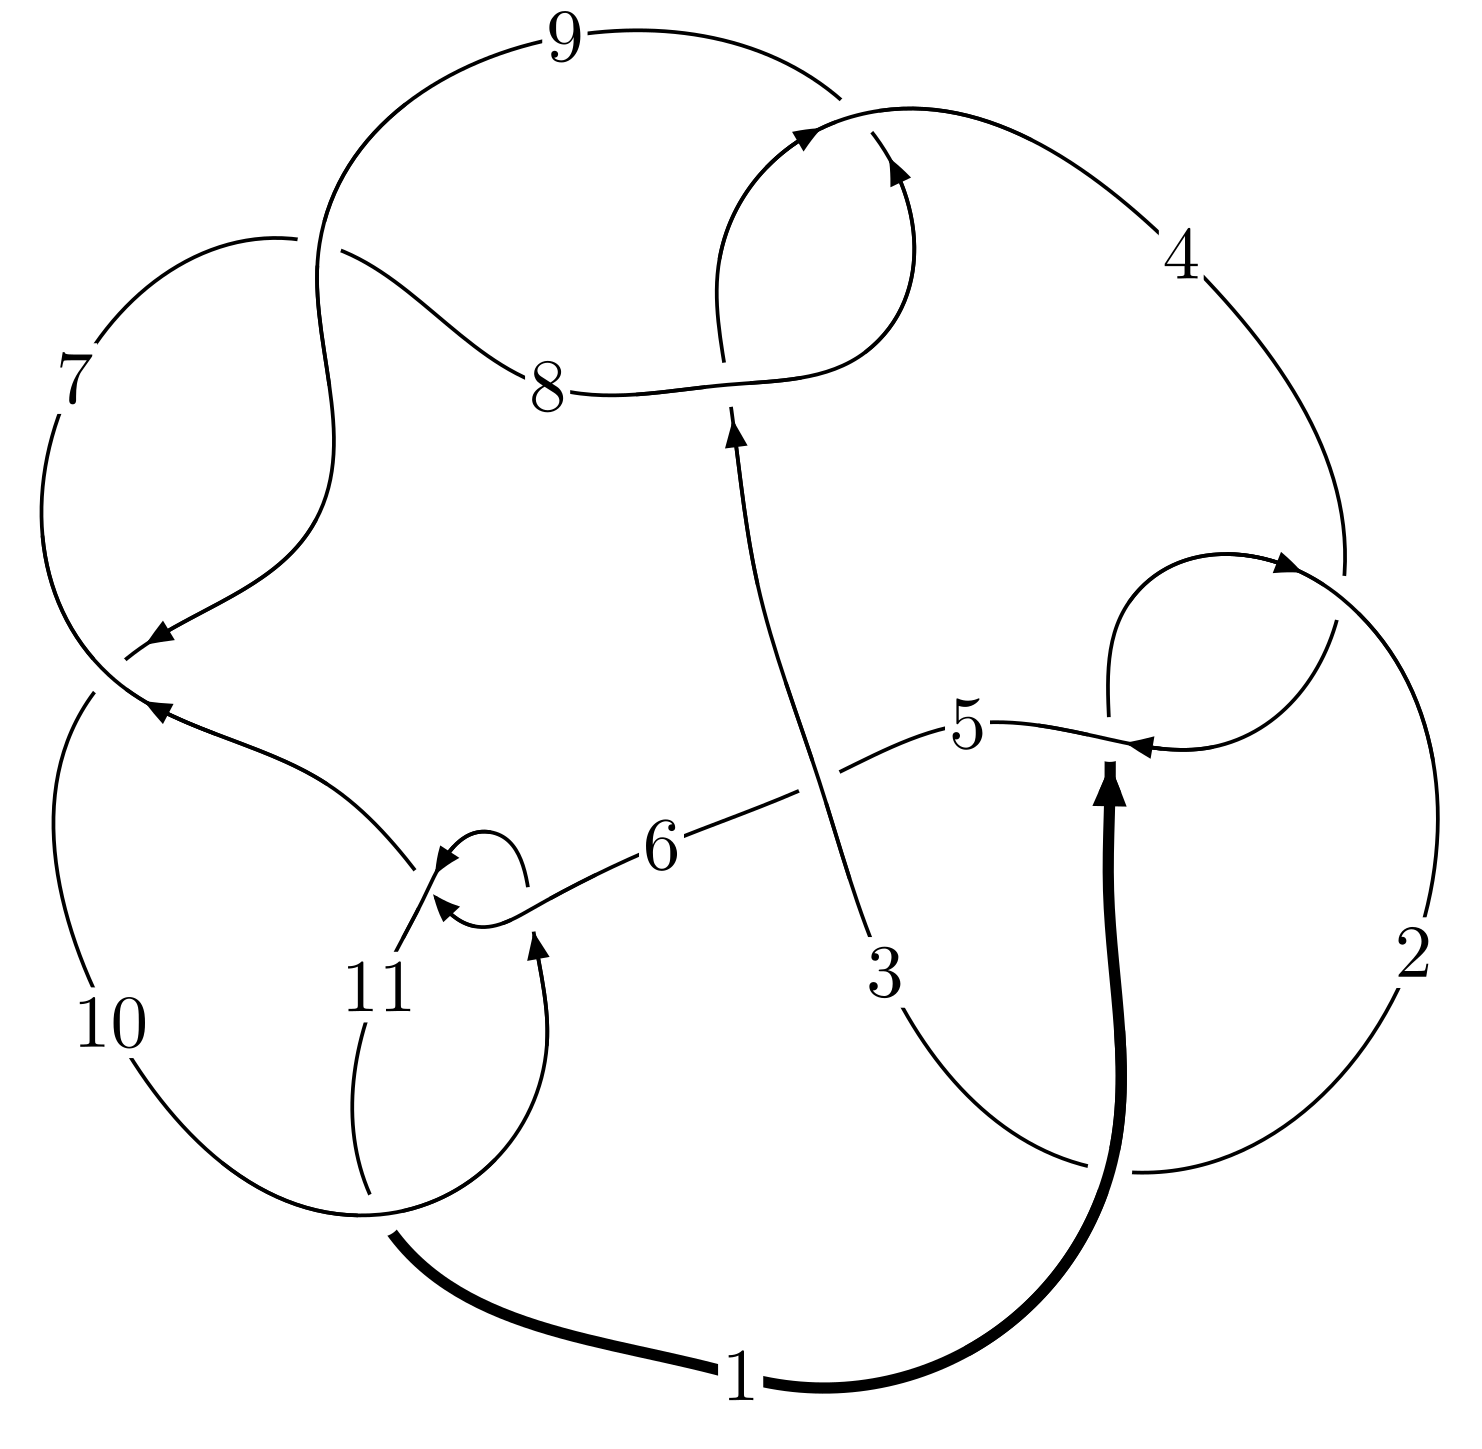
\includegraphics[width=112pt]{../../../GIT/diagram.site/Diagrams/png/260_11a_11.png}\\
\ \ \ A knot diagram\footnotemark}&
\allowdisplaybreaks
\textbf{Linearized knot diagam} \\
\cline{2-2}
 &
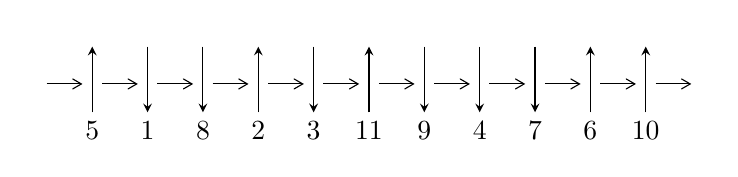
\begin{tikzpicture}[x=20pt, y=17pt]
	% nodes
	\node (C0) at (0, 0) {};
	\node (C1) at (1, 0) {};
	\node (C1U) at (1, +1) {};
	\node (C1D) at (1, -1) {5};

	\node (C2) at (2, 0) {};
	\node (C2U) at (2, +1) {};
	\node (C2D) at (2, -1) {1};

	\node (C3) at (3, 0) {};
	\node (C3U) at (3, +1) {};
	\node (C3D) at (3, -1) {8};

	\node (C4) at (4, 0) {};
	\node (C4U) at (4, +1) {};
	\node (C4D) at (4, -1) {2};

	\node (C5) at (5, 0) {};
	\node (C5U) at (5, +1) {};
	\node (C5D) at (5, -1) {3};

	\node (C6) at (6, 0) {};
	\node (C6U) at (6, +1) {};
	\node (C6D) at (6, -1) {11};

	\node (C7) at (7, 0) {};
	\node (C7U) at (7, +1) {};
	\node (C7D) at (7, -1) {9};

	\node (C8) at (8, 0) {};
	\node (C8U) at (8, +1) {};
	\node (C8D) at (8, -1) {4};

	\node (C9) at (9, 0) {};
	\node (C9U) at (9, +1) {};
	\node (C9D) at (9, -1) {7};

	\node (C10) at (10, 0) {};
	\node (C10U) at (10, +1) {};
	\node (C10D) at (10, -1) {6};

	\node (C11) at (11, 0) {};
	\node (C11U) at (11, +1) {};
	\node (C11D) at (11, -1) {10};
	\node (C12) at (12, 0) {};

	% arrows
	\draw[->,>={angle 60}]
	(C0) edge (C1) (C1) edge (C2) (C2) edge (C3) (C3) edge (C4) (C4) edge (C5) (C5) edge (C6) (C6) edge (C7) (C7) edge (C8) (C8) edge (C9) (C9) edge (C10) (C10) edge (C11) (C11) edge (C12) ;	\draw[->,>=stealth]
	(C1D) edge (C1U) (C2U) edge (C2D) (C3U) edge (C3D) (C4D) edge (C4U) (C5U) edge (C5D) (C6D) edge (C6U) (C7U) edge (C7D) (C8U) edge (C8D) (C9U) edge (C9D) (C10D) edge (C10U) (C11D) edge (C11U) ;
	\end{tikzpicture} \\
\hhline{~~} \\& 
\textbf{Solving Sequence} \\ \cline{2-2} 
 &
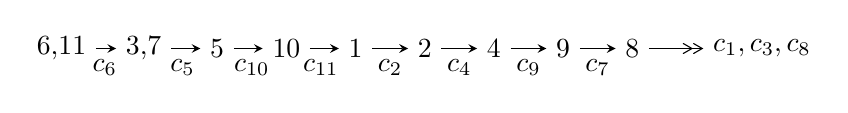
\begin{tikzpicture}[x=25pt, y=7pt]
	% node
	\node (A0) at (-1/8, 0) {6,11};
	\node (A1) at (17/16, 0) {3,7};
	\node (A2) at (17/8, 0) {5};
	\node (A3) at (25/8, 0) {10};
	\node (A4) at (33/8, 0) {1};
	\node (A5) at (41/8, 0) {2};
	\node (A6) at (49/8, 0) {4};
	\node (A7) at (57/8, 0) {9};
	\node (A8) at (65/8, 0) {8};
	\node (C1) at (1/2, -1) {$c_{6}$};
	\node (C2) at (13/8, -1) {$c_{5}$};
	\node (C3) at (21/8, -1) {$c_{10}$};
	\node (C4) at (29/8, -1) {$c_{11}$};
	\node (C5) at (37/8, -1) {$c_{2}$};
	\node (C6) at (45/8, -1) {$c_{4}$};
	\node (C7) at (53/8, -1) {$c_{9}$};
	\node (C8) at (61/8, -1) {$c_{7}$};
	\node (A9) at (10, 0) {$c_{1},c_{3},c_{8}$};

	% edge
	\draw[->,>=stealth]	
	(A0) edge (A1) (A1) edge (A2) (A2) edge (A3) (A3) edge (A4) (A4) edge (A5) (A5) edge (A6) (A6) edge (A7) (A7) edge (A8) ;
	\draw[->>,>={angle 60}]	
	(A8) edge (A9);
\end{tikzpicture} \\ 

\end{tabular} \\

\footnotetext{
The image of knot diagram is generated by the software ``\textbf{Draw programme}" developed by Andrew Bartholomew(\url{http://www.layer8.co.uk/maths/draw/index.htm\#Running-draw}), where we modified some parts for our purpose(\url{https://github.com/CATsTAILs/LinksPainter}).
}\phantom \\ \newline 
\centering \textbf{Ideals for irreducible components\footnotemark of $X_{\text{par}}$} 
 
\begin{align*}
I^u_{1}&=\langle 
5 u^{57}+12 u^{56}+\cdots+2 b+7,\;-13 u^{57}-30 u^{56}+\cdots+2 a-17,\;u^{58}+3 u^{57}+\cdots+2 u+1\rangle \\
I^u_{2}&=\langle 
b+a,\;a^2- a+1,\;u+1\rangle \\
\\
\end{align*}
\raggedright * 2 irreducible components of $\dim_{\mathbb{C}}=0$, with total 60 representations.\\
\footnotetext{All coefficients of polynomials are rational numbers. But the coefficients are sometimes approximated in decimal forms when there is not enough margin.}
\newpage
\renewcommand{\arraystretch}{1}
\centering \section*{I. $I^u_{1}= \langle 5 u^{57}+12 u^{56}+\cdots+2 b+7,\;-13 u^{57}-30 u^{56}+\cdots+2 a-17,\;u^{58}+3 u^{57}+\cdots+2 u+1 \rangle$}
\flushleft \textbf{(i) Arc colorings}\\
\begin{tabular}{m{7pt} m{180pt} m{7pt} m{180pt} }
\flushright $a_{6}=$&$\begin{pmatrix}1\\0\end{pmatrix}$ \\
\flushright $a_{11}=$&$\begin{pmatrix}0\\u\end{pmatrix}$ \\
\flushright $a_{3}=$&$\begin{pmatrix}\frac{13}{2} u^{57}+15 u^{56}+\cdots+\frac{21}{2} u+\frac{17}{2}\\-\frac{5}{2} u^{57}-6 u^{56}+\cdots-\frac{3}{2} u-\frac{7}{2}\end{pmatrix}$ \\
\flushright $a_{7}=$&$\begin{pmatrix}1\\- u^2\end{pmatrix}$ \\
\flushright $a_{5}=$&$\begin{pmatrix}-\frac{1}{2} u^{57}- u^{56}+\cdots+\frac{1}{2} u+\frac{3}{2}\\\frac{1}{2} u^{57}+u^{56}+\cdots+\frac{3}{2} u+\frac{1}{2}\end{pmatrix}$ \\
\flushright $a_{10}=$&$\begin{pmatrix}- u\\u\end{pmatrix}$ \\
\flushright $a_{1}=$&$\begin{pmatrix}u^3\\- u^3+u\end{pmatrix}$ \\
\flushright $a_{2}=$&$\begin{pmatrix}6 u^{57}+13 u^{56}+\cdots+10 u+7\\-\frac{9}{2} u^{57}-10 u^{56}+\cdots-\frac{7}{2} u-\frac{11}{2}\end{pmatrix}$ \\
\flushright $a_{4}=$&$\begin{pmatrix}\frac{9}{2} u^{57}+9 u^{56}+\cdots+\frac{13}{2} u+\frac{11}{2}\\-\frac{11}{2} u^{57}-12 u^{56}+\cdots-\frac{11}{2} u-\frac{13}{2}\end{pmatrix}$ \\
\flushright $a_{9}=$&$\begin{pmatrix}- u^3\\u^5- u^3+u\end{pmatrix}$ \\
\flushright $a_{8}=$&$\begin{pmatrix}u^6- u^4+1\\- u^8+2 u^6-2 u^4\end{pmatrix}$\\ \flushright $a_{8}=$&$\begin{pmatrix}u^6- u^4+1\\- u^8+2 u^6-2 u^4\end{pmatrix}$\\&\end{tabular}
\flushleft \textbf{(ii) Obstruction class $= -1$}\\~\\
\flushleft \textbf{(iii) Cusp Shapes $= 7 u^{57}+19 u^{56}+\cdots+5 u+8$}\\~\\
\newpage\renewcommand{\arraystretch}{1}
\flushleft \textbf{(iv) u-Polynomials at the component}\newline \\
\begin{tabular}{m{50pt}|m{274pt}}
Crossings & \hspace{64pt}u-Polynomials at each crossing \\
\hline $$\begin{aligned}c_{1},c_{4}\end{aligned}$$&$\begin{aligned}
&u^{58}+2 u^{57}+\cdots+3 u+1
\end{aligned}$\\
\hline $$\begin{aligned}c_{2}\end{aligned}$$&$\begin{aligned}
&u^{58}+26 u^{57}+\cdots+5 u+1
\end{aligned}$\\
\hline $$\begin{aligned}c_{3},c_{8}\end{aligned}$$&$\begin{aligned}
&u^{58}- u^{57}+\cdots+4 u+4
\end{aligned}$\\
\hline $$\begin{aligned}c_{5}\end{aligned}$$&$\begin{aligned}
&u^{58}-2 u^{57}+\cdots-5 u+1
\end{aligned}$\\
\hline $$\begin{aligned}c_{6},c_{10}\end{aligned}$$&$\begin{aligned}
&u^{58}+3 u^{57}+\cdots+2 u+1
\end{aligned}$\\
\hline $$\begin{aligned}c_{7},c_{9}\end{aligned}$$&$\begin{aligned}
&u^{58}+15 u^{57}+\cdots+168 u+16
\end{aligned}$\\
\hline $$\begin{aligned}c_{11}\end{aligned}$$&$\begin{aligned}
&u^{58}-33 u^{57}+\cdots+2 u+1
\end{aligned}$\\
\hline
\end{tabular}\\~\\
\newpage\renewcommand{\arraystretch}{1}
\flushleft \textbf{(v) Riley Polynomials at the component}\newline \\
\begin{tabular}{m{50pt}|m{274pt}}
Crossings & \hspace{64pt}Riley Polynomials at each crossing \\
\hline $$\begin{aligned}c_{1},c_{4}\end{aligned}$$&$\begin{aligned}
&y^{58}+26 y^{57}+\cdots+5 y+1
\end{aligned}$\\
\hline $$\begin{aligned}c_{2}\end{aligned}$$&$\begin{aligned}
&y^{58}+14 y^{57}+\cdots+29 y+1
\end{aligned}$\\
\hline $$\begin{aligned}c_{3},c_{8}\end{aligned}$$&$\begin{aligned}
&y^{58}-15 y^{57}+\cdots-168 y+16
\end{aligned}$\\
\hline $$\begin{aligned}c_{5}\end{aligned}$$&$\begin{aligned}
&y^{58}+2 y^{57}+\cdots+53 y+1
\end{aligned}$\\
\hline $$\begin{aligned}c_{6},c_{10}\end{aligned}$$&$\begin{aligned}
&y^{58}-33 y^{57}+\cdots+2 y+1
\end{aligned}$\\
\hline $$\begin{aligned}c_{7},c_{9}\end{aligned}$$&$\begin{aligned}
&y^{58}+53 y^{57}+\cdots+2784 y+256
\end{aligned}$\\
\hline $$\begin{aligned}c_{11}\end{aligned}$$&$\begin{aligned}
&y^{58}-13 y^{57}+\cdots+42 y+1
\end{aligned}$\\
\hline
\end{tabular}\\~\\
\newpage\flushleft \textbf{(vi) Complex Volumes and Cusp Shapes}
$$\begin{array}{c|c|c}  
\text{Solutions to }I^u_{1}& \I (\text{vol} + \sqrt{-1}CS) & \text{Cusp shape}\\
 \hline 
\begin{aligned}
u &= \phantom{-}0.936894 + 0.279112 I \\
a &= \phantom{-}1.047720 + 0.605690 I \\
b &= \phantom{-}0.369891 - 0.435412 I\end{aligned}
 & \phantom{-}1.77616 + 0.94992 I & \phantom{-}4.44755 - 1.71410 I \\ \hline\begin{aligned}
u &= \phantom{-}0.936894 - 0.279112 I \\
a &= \phantom{-}1.047720 - 0.605690 I \\
b &= \phantom{-}0.369891 + 0.435412 I\end{aligned}
 & \phantom{-}1.77616 - 0.94992 I & \phantom{-}4.44755 + 1.71410 I \\ \hline\begin{aligned}
u &= -0.916311 + 0.325300 I \\
a &= -0.44495 + 1.43722 I \\
b &= -0.115014 - 1.191470 I\end{aligned}
 & \phantom{-}1.56865 - 3.63401 I & \phantom{-}0.50067 + 8.81328 I \\ \hline\begin{aligned}
u &= -0.916311 - 0.325300 I \\
a &= -0.44495 - 1.43722 I \\
b &= -0.115014 + 1.191470 I\end{aligned}
 & \phantom{-}1.56865 + 3.63401 I & \phantom{-}0.50067 - 8.81328 I \\ \hline\begin{aligned}
u &= \phantom{-}0.879809 + 0.411472 I \\
a &= -1.87353 - 0.91118 I \\
b &= -0.963620 + 0.647776 I\end{aligned}
 & -0.11517 + 4.84774 I & -0.96980 - 7.14409 I \\ \hline\begin{aligned}
u &= \phantom{-}0.879809 - 0.411472 I \\
a &= -1.87353 + 0.91118 I \\
b &= -0.963620 - 0.647776 I\end{aligned}
 & -0.11517 - 4.84774 I & -0.96980 + 7.14409 I \\ \hline\begin{aligned}
u &= -0.872696 + 0.564700 I \\
a &= \phantom{-}0.11167 - 1.42828 I \\
b &= \phantom{-}0.724370 - 0.075036 I\end{aligned}
 & -4.33981 - 1.99854 I & -7.41077 + 3.19574 I \\ \hline\begin{aligned}
u &= -0.872696 - 0.564700 I \\
a &= \phantom{-}0.11167 + 1.42828 I \\
b &= \phantom{-}0.724370 + 0.075036 I\end{aligned}
 & -4.33981 + 1.99854 I & -7.41077 - 3.19574 I \\ \hline\begin{aligned}
u &= -0.961005 + 0.511826 I \\
a &= -0.391548 + 1.205530 I \\
b &= -0.865496 - 0.577881 I\end{aligned}
 & -0.45426 - 4.86179 I & \phantom{-0.000000 } 0 \\ \hline\begin{aligned}
u &= -0.961005 - 0.511826 I \\
a &= -0.391548 - 1.205530 I \\
b &= -0.865496 + 0.577881 I\end{aligned}
 & -0.45426 + 4.86179 I & \phantom{-0.000000 } 0\\
 \hline 
 \end{array}$$\newpage$$\begin{array}{c|c|c}  
\text{Solutions to }I^u_{1}& \I (\text{vol} + \sqrt{-1}CS) & \text{Cusp shape}\\
 \hline 
\begin{aligned}
u &= \phantom{-}1.091850 + 0.182421 I \\
a &= \phantom{-}0.618739 + 0.378922 I \\
b &= -0.033551 - 0.584136 I\end{aligned}
 & \phantom{-}2.16202 + 0.77457 I & \phantom{-0.000000 } 0 \\ \hline\begin{aligned}
u &= \phantom{-}1.091850 - 0.182421 I \\
a &= \phantom{-}0.618739 - 0.378922 I \\
b &= -0.033551 + 0.584136 I\end{aligned}
 & \phantom{-}2.16202 - 0.77457 I & \phantom{-0.000000 } 0 \\ \hline\begin{aligned}
u &= -0.114948 + 0.879124 I \\
a &= \phantom{-}0.293332 + 0.657468 I \\
b &= \phantom{-}1.34552 - 1.00402 I\end{aligned}
 & \phantom{-}2.14956 + 9.66192 I & -1.84579 - 7.09878 I \\ \hline\begin{aligned}
u &= -0.114948 - 0.879124 I \\
a &= \phantom{-}0.293332 - 0.657468 I \\
b &= \phantom{-}1.34552 + 1.00402 I\end{aligned}
 & \phantom{-}2.14956 - 9.66192 I & -1.84579 + 7.09878 I \\ \hline\begin{aligned}
u &= -0.847792 + 0.237371 I \\
a &= \phantom{-}1.00423 - 1.29055 I \\
b &= -0.610270 + 1.159360 I\end{aligned}
 & \phantom{-}1.09083 + 1.19632 I & -2.67942 + 2.86295 I \\ \hline\begin{aligned}
u &= -0.847792 - 0.237371 I \\
a &= \phantom{-}1.00423 + 1.29055 I \\
b &= -0.610270 - 1.159360 I\end{aligned}
 & \phantom{-}1.09083 - 1.19632 I & -2.67942 - 2.86295 I \\ \hline\begin{aligned}
u &= -0.620020 + 0.619213 I \\
a &= \phantom{-}0.637420 + 0.321223 I \\
b &= \phantom{-}0.877359 + 0.237702 I\end{aligned}
 & -5.05702 - 2.63543 I & -8.96800 + 3.93457 I \\ \hline\begin{aligned}
u &= -0.620020 - 0.619213 I \\
a &= \phantom{-}0.637420 - 0.321223 I \\
b &= \phantom{-}0.877359 - 0.237702 I\end{aligned}
 & -5.05702 + 2.63543 I & -8.96800 - 3.93457 I \\ \hline\begin{aligned}
u &= -0.089885 + 0.858078 I \\
a &= -0.112768 - 0.635694 I \\
b &= -0.786700 + 1.168860 I\end{aligned}
 & \phantom{-}4.07167 + 4.42773 I & \phantom{-}1.08988 - 2.76799 I \\ \hline\begin{aligned}
u &= -0.089885 - 0.858078 I \\
a &= -0.112768 + 0.635694 I \\
b &= -0.786700 - 1.168860 I\end{aligned}
 & \phantom{-}4.07167 - 4.42773 I & \phantom{-}1.08988 + 2.76799 I\\
 \hline 
 \end{array}$$\newpage$$\begin{array}{c|c|c}  
\text{Solutions to }I^u_{1}& \I (\text{vol} + \sqrt{-1}CS) & \text{Cusp shape}\\
 \hline 
\begin{aligned}
u &= -0.985848 + 0.568576 I \\
a &= \phantom{-}0.69359 - 1.33426 I \\
b &= \phantom{-}1.237080 + 0.630163 I\end{aligned}
 & -2.89029 - 9.39325 I & \phantom{-0.000000 } 0 \\ \hline\begin{aligned}
u &= -0.985848 - 0.568576 I \\
a &= \phantom{-}0.69359 + 1.33426 I \\
b &= \phantom{-}1.237080 - 0.630163 I\end{aligned}
 & -2.89029 + 9.39325 I & \phantom{-0.000000 } 0 \\ \hline\begin{aligned}
u &= -0.468879 + 0.677261 I \\
a &= \phantom{-}0.599662 - 0.565289 I \\
b &= \phantom{-}1.104110 - 0.515806 I\end{aligned}
 & -4.36361 + 4.61978 I & -7.52611 - 4.69531 I \\ \hline\begin{aligned}
u &= -0.468879 - 0.677261 I \\
a &= \phantom{-}0.599662 + 0.565289 I \\
b &= \phantom{-}1.104110 + 0.515806 I\end{aligned}
 & -4.36361 - 4.61978 I & -7.52611 + 4.69531 I \\ \hline\begin{aligned}
u &= -0.008417 + 0.809874 I \\
a &= \phantom{-}0.341800 - 0.733041 I \\
b &= \phantom{-}0.587922 + 1.243870 I\end{aligned}
 & \phantom{-}4.43701 + 1.53415 I & \phantom{-}1.72366 - 2.51421 I \\ \hline\begin{aligned}
u &= -0.008417 - 0.809874 I \\
a &= \phantom{-}0.341800 + 0.733041 I \\
b &= \phantom{-}0.587922 - 1.243870 I\end{aligned}
 & \phantom{-}4.43701 - 1.53415 I & \phantom{-}1.72366 + 2.51421 I \\ \hline\begin{aligned}
u &= \phantom{-}1.191990 + 0.080409 I \\
a &= -0.975096 - 0.416483 I \\
b &= \phantom{-}0.809328 + 0.659275 I\end{aligned}
 & \phantom{-}0.90066 - 2.88860 I & \phantom{-0.000000 } 0 \\ \hline\begin{aligned}
u &= \phantom{-}1.191990 - 0.080409 I \\
a &= -0.975096 + 0.416483 I \\
b &= \phantom{-}0.809328 - 0.659275 I\end{aligned}
 & \phantom{-}0.90066 + 2.88860 I & \phantom{-0.000000 } 0 \\ \hline\begin{aligned}
u &= \phantom{-}0.038017 + 0.792195 I \\
a &= -0.558913 + 0.868902 I \\
b &= -1.20038 - 1.07211 I\end{aligned}
 & \phantom{-}2.81999 - 3.64889 I & -0.72605 + 2.41695 I \\ \hline\begin{aligned}
u &= \phantom{-}0.038017 - 0.792195 I \\
a &= -0.558913 - 0.868902 I \\
b &= -1.20038 + 1.07211 I\end{aligned}
 & \phantom{-}2.81999 + 3.64889 I & -0.72605 - 2.41695 I\\
 \hline 
 \end{array}$$\newpage$$\begin{array}{c|c|c}  
\text{Solutions to }I^u_{1}& \I (\text{vol} + \sqrt{-1}CS) & \text{Cusp shape}\\
 \hline 
\begin{aligned}
u &= -0.135832 + 0.774619 I \\
a &= \phantom{-}0.029723 + 0.956439 I \\
b &= \phantom{-}0.224876 - 0.143157 I\end{aligned}
 & -1.07636 + 2.53447 I & -5.45479 - 2.49966 I \\ \hline\begin{aligned}
u &= -0.135832 - 0.774619 I \\
a &= \phantom{-}0.029723 - 0.956439 I \\
b &= \phantom{-}0.224876 + 0.143157 I\end{aligned}
 & -1.07636 - 2.53447 I & -5.45479 + 2.49966 I \\ \hline\begin{aligned}
u &= \phantom{-}1.181050 + 0.400971 I \\
a &= -0.091410 - 1.158760 I \\
b &= -0.061904 + 0.135595 I\end{aligned}
 & \phantom{-}2.74272 + 1.35672 I & \phantom{-0.000000 } 0 \\ \hline\begin{aligned}
u &= \phantom{-}1.181050 - 0.400971 I \\
a &= -0.091410 + 1.158760 I \\
b &= -0.061904 - 0.135595 I\end{aligned}
 & \phantom{-}2.74272 - 1.35672 I & \phantom{-0.000000 } 0 \\ \hline\begin{aligned}
u &= \phantom{-}0.653392 + 0.334802 I \\
a &= -0.95931 - 1.89944 I \\
b &= -0.695507 - 0.477939 I\end{aligned}
 & -0.81275 - 1.40752 I & -3.05190 + 0.70072 I \\ \hline\begin{aligned}
u &= \phantom{-}0.653392 - 0.334802 I \\
a &= -0.95931 + 1.89944 I \\
b &= -0.695507 + 0.477939 I\end{aligned}
 & -0.81275 + 1.40752 I & -3.05190 - 0.70072 I \\ \hline\begin{aligned}
u &= -0.480577 + 0.547338 I \\
a &= -0.133346 + 0.235167 I \\
b &= -0.763916 + 0.261710 I\end{aligned}
 & -1.79712 + 0.58239 I & -4.29390 - 0.53701 I \\ \hline\begin{aligned}
u &= -0.480577 - 0.547338 I \\
a &= -0.133346 - 0.235167 I \\
b &= -0.763916 - 0.261710 I\end{aligned}
 & -1.79712 - 0.58239 I & -4.29390 + 0.53701 I \\ \hline\begin{aligned}
u &= -1.211310 + 0.439886 I \\
a &= \phantom{-}1.64164 - 0.97222 I \\
b &= -1.21429 + 1.19635 I\end{aligned}
 & \phantom{-}6.48025 - 0.70893 I & \phantom{-0.000000 } 0 \\ \hline\begin{aligned}
u &= -1.211310 - 0.439886 I \\
a &= \phantom{-}1.64164 + 0.97222 I \\
b &= -1.21429 - 1.19635 I\end{aligned}
 & \phantom{-}6.48025 + 0.70893 I & \phantom{-0.000000 } 0\\
 \hline 
 \end{array}$$\newpage$$\begin{array}{c|c|c}  
\text{Solutions to }I^u_{1}& \I (\text{vol} + \sqrt{-1}CS) & \text{Cusp shape}\\
 \hline 
\begin{aligned}
u &= -1.188910 + 0.500899 I \\
a &= \phantom{-}0.126269 - 1.350040 I \\
b &= \phantom{-}0.214574 + 0.310119 I\end{aligned}
 & \phantom{-}2.01751 - 7.25755 I & \phantom{-0.000000 } 0 \\ \hline\begin{aligned}
u &= -1.188910 - 0.500899 I \\
a &= \phantom{-}0.126269 + 1.350040 I \\
b &= \phantom{-}0.214574 - 0.310119 I\end{aligned}
 & \phantom{-}2.01751 + 7.25755 I & \phantom{-0.000000 } 0 \\ \hline\begin{aligned}
u &= \phantom{-}1.207870 + 0.472373 I \\
a &= -0.30001 - 2.69705 I \\
b &= -1.30956 + 1.04786 I\end{aligned}
 & \phantom{-}6.24695 + 8.22888 I & \phantom{-0.000000 } 0 \\ \hline\begin{aligned}
u &= \phantom{-}1.207870 - 0.472373 I \\
a &= -0.30001 + 2.69705 I \\
b &= -1.30956 - 1.04786 I\end{aligned}
 & \phantom{-}6.24695 - 8.22888 I & \phantom{-0.000000 } 0 \\ \hline\begin{aligned}
u &= \phantom{-}1.218760 + 0.453390 I \\
a &= \phantom{-}0.67289 + 2.30853 I \\
b &= \phantom{-}0.72918 - 1.22228 I\end{aligned}
 & \phantom{-}8.06195 + 2.97069 I & \phantom{-0.000000 } 0 \\ \hline\begin{aligned}
u &= \phantom{-}1.218760 - 0.453390 I \\
a &= \phantom{-}0.67289 - 2.30853 I \\
b &= \phantom{-}0.72918 + 1.22228 I\end{aligned}
 & \phantom{-}8.06195 - 2.97069 I & \phantom{-0.000000 } 0 \\ \hline\begin{aligned}
u &= -1.217390 + 0.461266 I \\
a &= -1.34002 + 1.45284 I \\
b &= \phantom{-}0.58894 - 1.38167 I\end{aligned}
 & \phantom{-}8.00524 - 6.08837 I & \phantom{-0.000000 } 0 \\ \hline\begin{aligned}
u &= -1.217390 - 0.461266 I \\
a &= -1.34002 - 1.45284 I \\
b &= \phantom{-}0.58894 + 1.38167 I\end{aligned}
 & \phantom{-}8.00524 + 6.08837 I & \phantom{-0.000000 } 0 \\ \hline\begin{aligned}
u &= \phantom{-}1.249820 + 0.409605 I \\
a &= \phantom{-}1.42176 + 1.29568 I \\
b &= -0.67640 - 1.24410 I\end{aligned}
 & \phantom{-}8.16003 - 0.02626 I & \phantom{-0.000000 } 0 \\ \hline\begin{aligned}
u &= \phantom{-}1.249820 - 0.409605 I \\
a &= \phantom{-}1.42176 - 1.29568 I \\
b &= -0.67640 + 1.24410 I\end{aligned}
 & \phantom{-}8.16003 + 0.02626 I & \phantom{-0.000000 } 0\\
 \hline 
 \end{array}$$\newpage$$\begin{array}{c|c|c}  
\text{Solutions to }I^u_{1}& \I (\text{vol} + \sqrt{-1}CS) & \text{Cusp shape}\\
 \hline 
\begin{aligned}
u &= \phantom{-}1.264910 + 0.391892 I \\
a &= -1.67105 - 0.82125 I \\
b &= \phantom{-}1.27143 + 1.06896 I\end{aligned}
 & \phantom{-}6.42683 - 5.27485 I & \phantom{-0.000000 } 0 \\ \hline\begin{aligned}
u &= \phantom{-}1.264910 - 0.391892 I \\
a &= -1.67105 + 0.82125 I \\
b &= \phantom{-}1.27143 - 1.06896 I\end{aligned}
 & \phantom{-}6.42683 + 5.27485 I & \phantom{-0.000000 } 0 \\ \hline\begin{aligned}
u &= -1.225810 + 0.504607 I \\
a &= -0.43554 + 2.29097 I \\
b &= -0.86675 - 1.23626 I\end{aligned}
 & \phantom{-}7.47129 - 9.35808 I & \phantom{-0.000000 } 0 \\ \hline\begin{aligned}
u &= -1.225810 - 0.504607 I \\
a &= -0.43554 - 2.29097 I \\
b &= -0.86675 + 1.23626 I\end{aligned}
 & \phantom{-}7.47129 + 9.35808 I & \phantom{-0.000000 } 0 \\ \hline\begin{aligned}
u &= -1.228790 + 0.519584 I \\
a &= \phantom{-}0.05132 - 2.55286 I \\
b &= \phantom{-}1.40940 + 1.03866 I\end{aligned}
 & \phantom{-}5.5002 - 14.7239 I & \phantom{-0.000000 } 0 \\ \hline\begin{aligned}
u &= -1.228790 - 0.519584 I \\
a &= \phantom{-}0.05132 + 2.55286 I \\
b &= \phantom{-}1.40940 - 1.03866 I\end{aligned}
 & \phantom{-}5.5002 + 14.7239 I & \phantom{-0.000000 } 0 \\ \hline\begin{aligned}
u &= \phantom{-}0.160056 + 0.305941 I \\
a &= \phantom{-}0.49573 + 2.06046 I \\
b &= -0.330626 + 0.576257 I\end{aligned}
 & -0.32061 + 1.54716 I & -2.16073 - 4.65280 I \\ \hline\begin{aligned}
u &= \phantom{-}0.160056 - 0.305941 I \\
a &= \phantom{-}0.49573 - 2.06046 I \\
b &= -0.330626 - 0.576257 I\end{aligned}
 & -0.32061 - 1.54716 I & -2.16073 + 4.65280 I\\
 \hline 
 \end{array}$$\newpage\newpage\renewcommand{\arraystretch}{1}
\centering \section*{II. $I^u_{2}= \langle b+a,\;a^2- a+1,\;u+1 \rangle$}
\flushleft \textbf{(i) Arc colorings}\\
\begin{tabular}{m{7pt} m{180pt} m{7pt} m{180pt} }
\flushright $a_{6}=$&$\begin{pmatrix}1\\0\end{pmatrix}$ \\
\flushright $a_{11}=$&$\begin{pmatrix}0\\-1\end{pmatrix}$ \\
\flushright $a_{3}=$&$\begin{pmatrix}a\\- a\end{pmatrix}$ \\
\flushright $a_{7}=$&$\begin{pmatrix}1\\-1\end{pmatrix}$ \\
\flushright $a_{5}=$&$\begin{pmatrix}a\\- a+1\end{pmatrix}$ \\
\flushright $a_{10}=$&$\begin{pmatrix}1\\-1\end{pmatrix}$ \\
\flushright $a_{1}=$&$\begin{pmatrix}-1\\0\end{pmatrix}$ \\
\flushright $a_{2}=$&$\begin{pmatrix}0\\- a\end{pmatrix}$ \\
\flushright $a_{4}=$&$\begin{pmatrix}a\\- a\end{pmatrix}$ \\
\flushright $a_{9}=$&$\begin{pmatrix}1\\-1\end{pmatrix}$ \\
\flushright $a_{8}=$&$\begin{pmatrix}1\\-1\end{pmatrix}$\\ \flushright $a_{8}=$&$\begin{pmatrix}1\\-1\end{pmatrix}$\\&\end{tabular}
\flushleft \textbf{(ii) Obstruction class $= 1$}\\~\\
\flushleft \textbf{(iii) Cusp Shapes $= 4 a+1$}\\~\\
\newpage\renewcommand{\arraystretch}{1}
\flushleft \textbf{(iv) u-Polynomials at the component}\newline \\
\begin{tabular}{m{50pt}|m{274pt}}
Crossings & \hspace{64pt}u-Polynomials at each crossing \\
\hline $$\begin{aligned}c_{1},c_{2},c_{5}\end{aligned}$$&$\begin{aligned}
&u^2+u+1
\end{aligned}$\\
\hline $$\begin{aligned}c_{3},c_{7},c_{8}\\c_{9}\end{aligned}$$&$\begin{aligned}
&u^2
\end{aligned}$\\
\hline $$\begin{aligned}c_{4}\end{aligned}$$&$\begin{aligned}
&u^2- u+1
\end{aligned}$\\
\hline $$\begin{aligned}c_{6}\end{aligned}$$&$\begin{aligned}
&(u+1)^2
\end{aligned}$\\
\hline $$\begin{aligned}c_{10},c_{11}\end{aligned}$$&$\begin{aligned}
&(u-1)^2
\end{aligned}$\\
\hline
\end{tabular}\\~\\
\newpage\renewcommand{\arraystretch}{1}
\flushleft \textbf{(v) Riley Polynomials at the component}\newline \\
\begin{tabular}{m{50pt}|m{274pt}}
Crossings & \hspace{64pt}Riley Polynomials at each crossing \\
\hline $$\begin{aligned}c_{1},c_{2},c_{4}\\c_{5}\end{aligned}$$&$\begin{aligned}
&y^2+y+1
\end{aligned}$\\
\hline $$\begin{aligned}c_{3},c_{7},c_{8}\\c_{9}\end{aligned}$$&$\begin{aligned}
&y^2
\end{aligned}$\\
\hline $$\begin{aligned}c_{6},c_{10},c_{11}\end{aligned}$$&$\begin{aligned}
&(y-1)^2
\end{aligned}$\\
\hline
\end{tabular}\\~\\
\newpage\flushleft \textbf{(vi) Complex Volumes and Cusp Shapes}
$$\begin{array}{c|c|c}  
\text{Solutions to }I^u_{2}& \I (\text{vol} + \sqrt{-1}CS) & \text{Cusp shape}\\
 \hline 
\begin{aligned}
u &= -1.00000\phantom{ +0.000000I} \\
a &= \phantom{-}0.500000 + 0.866025 I \\
b &= -0.500000 - 0.866025 I\end{aligned}
 & \phantom{-}1.64493 - 2.02988 I & \phantom{-}3.00000 + 3.46410 I \\ \hline\begin{aligned}
u &= -1.00000\phantom{ +0.000000I} \\
a &= \phantom{-}0.500000 - 0.866025 I \\
b &= -0.500000 + 0.866025 I\end{aligned}
 & \phantom{-}1.64493 + 2.02988 I & \phantom{-}3.00000 - 3.46410 I\\
 \hline 
 \end{array}$$\newpage
\newpage\renewcommand{\arraystretch}{1}
\centering \section*{ III. u-Polynomials}
\begin{tabular}{m{50pt}|m{274pt}}
Crossings & \hspace{64pt}u-Polynomials at each crossing \\
\hline $$\begin{aligned}c_{1}\end{aligned}$$&$\begin{aligned}
&(u^2+u+1)(u^{58}+2 u^{57}+\cdots+3 u+1)
\end{aligned}$\\
\hline $$\begin{aligned}c_{2}\end{aligned}$$&$\begin{aligned}
&(u^2+u+1)(u^{58}+26 u^{57}+\cdots+5 u+1)
\end{aligned}$\\
\hline $$\begin{aligned}c_{3},c_{8}\end{aligned}$$&$\begin{aligned}
&u^2(u^{58}- u^{57}+\cdots+4 u+4)
\end{aligned}$\\
\hline $$\begin{aligned}c_{4}\end{aligned}$$&$\begin{aligned}
&(u^2- u+1)(u^{58}+2 u^{57}+\cdots+3 u+1)
\end{aligned}$\\
\hline $$\begin{aligned}c_{5}\end{aligned}$$&$\begin{aligned}
&(u^2+u+1)(u^{58}-2 u^{57}+\cdots-5 u+1)
\end{aligned}$\\
\hline $$\begin{aligned}c_{6}\end{aligned}$$&$\begin{aligned}
&((u+1)^2)(u^{58}+3 u^{57}+\cdots+2 u+1)
\end{aligned}$\\
\hline $$\begin{aligned}c_{7},c_{9}\end{aligned}$$&$\begin{aligned}
&u^2(u^{58}+15 u^{57}+\cdots+168 u+16)
\end{aligned}$\\
\hline $$\begin{aligned}c_{10}\end{aligned}$$&$\begin{aligned}
&((u-1)^2)(u^{58}+3 u^{57}+\cdots+2 u+1)
\end{aligned}$\\
\hline $$\begin{aligned}c_{11}\end{aligned}$$&$\begin{aligned}
&((u-1)^2)(u^{58}-33 u^{57}+\cdots+2 u+1)
\end{aligned}$\\
\hline
\end{tabular}\newpage\renewcommand{\arraystretch}{1}
\centering \section*{ IV. Riley Polynomials}
\begin{tabular}{m{50pt}|m{274pt}}
Crossings & \hspace{64pt}Riley Polynomials at each crossing \\
\hline $$\begin{aligned}c_{1},c_{4}\end{aligned}$$&$\begin{aligned}
&(y^2+y+1)(y^{58}+26 y^{57}+\cdots+5 y+1)
\end{aligned}$\\
\hline $$\begin{aligned}c_{2}\end{aligned}$$&$\begin{aligned}
&(y^2+y+1)(y^{58}+14 y^{57}+\cdots+29 y+1)
\end{aligned}$\\
\hline $$\begin{aligned}c_{3},c_{8}\end{aligned}$$&$\begin{aligned}
&y^2(y^{58}-15 y^{57}+\cdots-168 y+16)
\end{aligned}$\\
\hline $$\begin{aligned}c_{5}\end{aligned}$$&$\begin{aligned}
&(y^2+y+1)(y^{58}+2 y^{57}+\cdots+53 y+1)
\end{aligned}$\\
\hline $$\begin{aligned}c_{6},c_{10}\end{aligned}$$&$\begin{aligned}
&((y-1)^2)(y^{58}-33 y^{57}+\cdots+2 y+1)
\end{aligned}$\\
\hline $$\begin{aligned}c_{7},c_{9}\end{aligned}$$&$\begin{aligned}
&y^2(y^{58}+53 y^{57}+\cdots+2784 y+256)
\end{aligned}$\\
\hline $$\begin{aligned}c_{11}\end{aligned}$$&$\begin{aligned}
&((y-1)^2)(y^{58}-13 y^{57}+\cdots+42 y+1)
\end{aligned}$\\
\hline
\end{tabular}
\vskip 2pc
\end{document}